
\noindent\textbf{2. (CRLS Ex. 22.2-2)} Simule o funcionamento da \proc{BFS} no grafo da Figura 22.3 do CLRS (segunda
edição) a partir do vértice $u$, determinando os valores de $d$ e $\pi$ para cada vértice.

\textbf{Resposta:} A mesma analogia aplicada na questão anterior pode ser utilizada aqui, mesmo tratando-se de um grafo não orientado, o algoritmo \proc{BFS} funciona em ambos os casos, conforme vimos em sala/CLRS.

\begin{center}
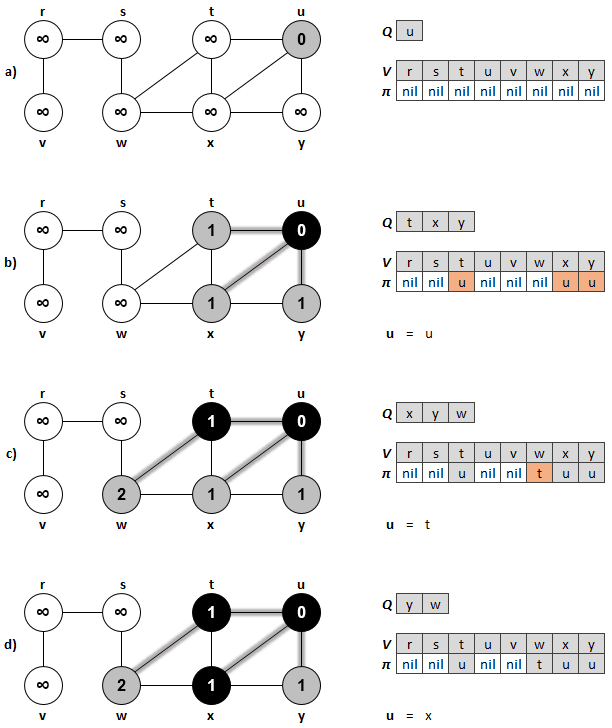
\includegraphics[width=0.8\textwidth]{q7-02-p1.png}
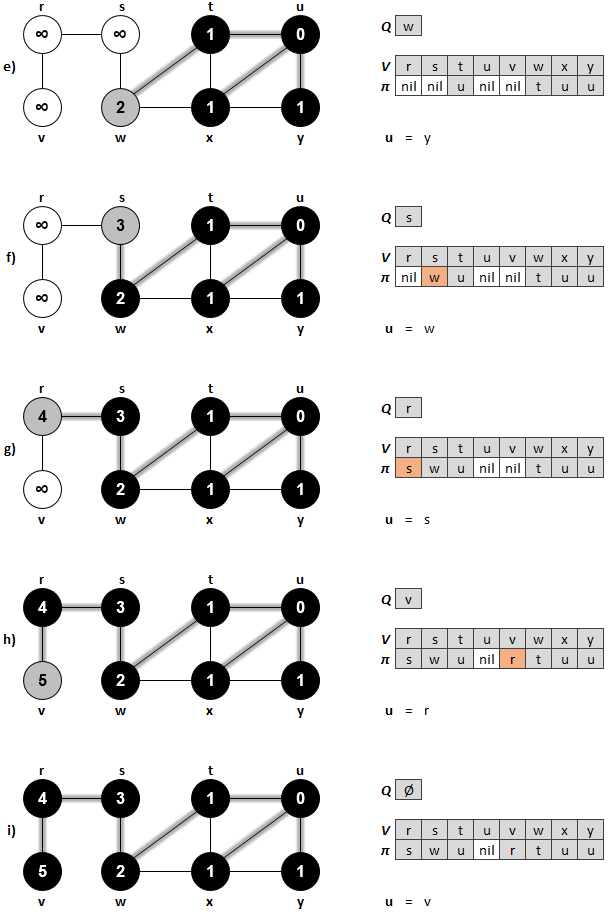
\includegraphics[width=0.8\textwidth]{q7-02-p2.png}
\captionof{figure}{Sequência das operações do algoritmo \proc{BFS}, sendo $s = u$.}
\label{fig:7.2-1}
\end{center}